\documentclass[11pt,a4paper]{article}
\usepackage[utf8]{inputenc}
\usepackage[T1]{fontenc}
\usepackage[french]{babel}
\usepackage{amsmath,amssymb}
\usepackage{graphicx}
\usepackage{booktabs}
\usepackage[margin=2.3cm]{geometry}
\usepackage{enumitem}
\setlist{itemsep=2pt,topsep=3pt}
\title{Pourquoi le gradient spectral oscille autour d'un bord net}
\author{Célian Baffalie -- Projet IMA (édition d'image dans le domaine spectral)}
\date{}
\begin{document}
\maketitle
\section*{Objectif}
Dans les tests, le gradient calculé par la méthode de l'article (éq. 13) présente des oscillations autour des bords nets, alors que le gradient aux différences finies n'en présente pas. Ce document explique ce phénomène uniquement à partir de la formule du gradient spectral, sur le cas le plus simple : une ligne d'image qui contient un saut.

\section*{Cadre et notations}
On travaille sur une seule ligne de l'image.

\begin{itemize}
\item \textbf{Pixels.} Les pixels sont repérés par un entier $k \in \mathbb{Z}$. On note $f[k]$ le niveau de gris du pixel $k$. On suppose la ligne très longue, pour ne pas s'occuper de ses extrémités (le code travaille sur une ligne finie prolongée par miroir ; loin des extrémités, le résultat est le même).
\item \textbf{Ondes.} Pour un réel $w$, on appelle \emph{onde de pulsation} $w$ la suite $k \mapsto e^{iwk}$. Comme $e^{i(w+2\pi)k} = e^{iwk}$ pour tout entier $k$, deux pulsations qui diffèrent de $2\pi$ donnent la même onde sur les pixels : il suffit de considérer $w \in [-\pi, \pi]$. La pulsation $w = 0$ donne une onde constante ; $w = \pi$ donne $e^{i\pi k} = (-1)^k$, l'onde la plus rapide possible sur la grille.
\item \textbf{Transformée de Fourier.} Le coefficient de Fourier de $f$ à la pulsation $w$ est
\end{itemize}
\begin{equation}
\hat{f}(w) = \sum_{k} f[k]\, e^{-iwk}
\end{equation}
et on retrouve $f$ à partir de ses coefficients par la formule inverse

\begin{equation}
f[k] = \frac{1}{2\pi} \int_{-\pi}^{\pi} \hat{f}(w)\, e^{iwk}\, dw .
\end{equation}
La formule (2) dit que $f$ est une \emph{somme d'ondes} : $\hat{f}(w)$ est le poids de l'onde de pulsation $w$ dans $f$. Dans le code, la FFT calcule ces poids aux pulsations $w_m = 2\pi m / N$ (avec $m$ ramené entre $-N/2$ et $N/2$ : c'est le recentrage), et l'intégrale devient une somme ; pour une ligne longue, cela revient au même.

\section*{Les deux gradients à comparer}
\begin{itemize}
\item \textbf{Gradient spectral.} Dériver l'onde $e^{iwx}$ donne $iw\, e^{iwx}$. L'éq. 13 de l'article dérive donc $f$ en multipliant chaque poids par $iw$ :
\end{itemize}
\begin{equation}
\hat{V}(w) = iw\, \hat{f}(w), \qquad V[k] = \frac{1}{2\pi} \int_{-\pi}^{\pi} iw\, \hat{f}(w)\, e^{iwk}\, dw .
\end{equation}
$V[k]$ est ce que calcule le code (\emph{gradient\_hat} puis transformée inverse).

\begin{itemize}
\item \textbf{Différence finie.}
\end{itemize}
\begin{equation}
D[k] = f[k+1] - f[k] .
\end{equation}
\section*{Deux outils}
\textbf{Outil 1 (décalage d'un pixel).} Si $g[k] = f[k-1]$ ($f$ décalé d'un pixel vers la droite), alors $\hat{g}(w) = e^{-iw}\, \hat{f}(w)$. En effet, en posant $j = k - 1$ :

\[
\hat{g}(w) = \sum_k f[k-1]\, e^{-iwk} = \sum_j f[j]\, e^{-iw(j+1)} = e^{-iw}\, \hat{f}(w) .
\]
De même, $f[k+1]$ a pour coefficients $e^{iw}\, \hat{f}(w)$.

\textbf{Outil 2 (somme de toutes les ondes).} Pour tout réel $t \neq 0$ :

\begin{equation}
\frac{1}{2\pi} \int_{-\pi}^{\pi} e^{iwt}\, dw = \frac{1}{2\pi}\, \frac{e^{i\pi t} - e^{-i\pi t}}{it} = \frac{\sin(\pi t)}{\pi t} ,
\end{equation}
et cette intégrale vaut 1 en $t = 0$. On en tire deux cas qui vont tout expliquer :

\begin{itemize}
\item si $t$ est un \textbf{entier non nul}, $\sin(\pi t) = 0$ : l'intégrale est \textbf{nulle} ;
\item si $t = k + \frac{1}{2}$ est un \textbf{demi-entier}, $\sin(\pi(k + \frac{1}{2})) = (-1)^k$ : l'intégrale vaut $\frac{(-1)^k}{\pi (k + 1/2)}$, qui \textbf{n'est jamais nulle}.
\end{itemize}
Autrement dit : additionner toutes les ondes de $-\pi$ à $\pi$ avec le même poids donne un pic en $t = 0$. À une distance entière du pic, les ondes se compensent exactement ; à une distance demi-entière, elles ne se compensent pas.

\section*{Le signal étudié : un saut}
\begin{equation}
f[k] = 0 \ \ \mathrm{si}\ k \leq -1, \qquad f[k] = H \ \ \mathrm{si}\ k \geq 0 .
\end{equation}
Le saut, de hauteur $H$, se trouve \textbf{entre} les pixels $-1$ et $0$, c'est-à-dire à la position $-\frac{1}{2}$. Le pixel $k$ est donc à la distance $k + \frac{1}{2}$ du saut. Dans les tests, $H = 150$.

\section*{Étape 1 : les coefficients de Fourier du saut}
On considère les différences $d[k] = f[k] - f[k-1]$. Elles sont toutes nulles, sauf $d[0] = H$. La somme (1) ne contient donc qu'un terme : $\hat{d}(w) = H$. Par ailleurs $d$ est la différence entre $f$ et $f$ décalé d'un pixel, donc d'après l'outil 1, $\hat{d}(w) = (1 - e^{-iw})\, \hat{f}(w)$. On en déduit :

\begin{equation}
\hat{f}(w) = \frac{H}{1 - e^{-iw}} \qquad (w \neq 0) .
\end{equation}
(En $w = 0$, la somme (1) diverge car le saut ne revient jamais à 0 ; ce point disparaît à l'étape suivante, où l'on multiplie par $iw$.)

\section*{Étape 2 : les coefficients du gradient spectral}
On multiplie par $iw$ comme dans (3), puis on factorise le dénominateur par $e^{-iw/2}$ :

\[
1 - e^{-iw} = e^{-iw/2}\left(e^{iw/2} - e^{-iw/2}\right) = 2i\, \sin(w/2)\, e^{-iw/2} .
\]
On obtient :

\begin{equation}
\hat{V}(w) = \frac{iw\, H}{1 - e^{-iw}} = H\, A(w)\, e^{iw/2}, \qquad A(w) = \frac{w/2}{\sin(w/2)} .
\end{equation}
Ce résultat se lit en deux morceaux :

\begin{itemize}
\item \textbf{$A(w)$ est la taille des poids.} Elle vaut 1 pour $w$ proche de 0 et $\pi/2 \approx 1{,}57$ pour $w = \pi$ : elle est \textbf{presque constante}. Toutes les ondes, des plus lentes aux plus rapides, ont presque le même poids dans le gradient. C'est attendu : la dérivée d'un saut est un pic, et un pic contient toutes les fréquences.
\item \textbf{$e^{iw/2}$ est un décalage d'un demi-pixel.} D'après l'outil 1, multiplier par $e^{iw/2}$ revient à décaler d'un demi-pixel vers la gauche : le pic est centré en $-\frac{1}{2}$, à l'endroit du saut, \textbf{entre deux pixels}.
\end{itemize}
\begin{figure}[h]
\centering
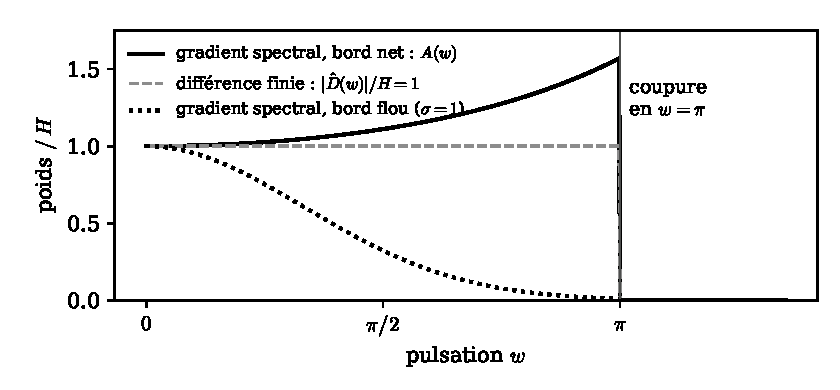
\includegraphics[width=0.78\textwidth]{figures/poids.pdf}
\caption{Taille des poids des ondes en fonction de la pulsation $w$. Pour un bord net, les poids du gradient spectral restent presque constants puis sont coupés brutalement en $w = \pi$ ; pour un bord flou, ils décroissent jusqu'à presque zéro avant $\pi$.}
\end{figure}
\section*{Étape 3 : retour aux pixels}
On remet (8) dans la formule inverse (2) :

\begin{equation}
V[k] = \frac{1}{2\pi} \int_{-\pi}^{\pi} H\, A(w)\, e^{iw/2}\, e^{iwk}\, dw = \frac{H}{2\pi} \int_{-\pi}^{\pi} A(w)\, e^{iw(k + 1/2)}\, dw .
\end{equation}
La distance $k + \frac{1}{2}$ entre le pixel et le saut apparaît. Si l'on remplace $A(w)$ par 1 (poids constants), l'outil 2 avec $t = k + \frac{1}{2}$ donne directement :

\begin{equation}
V[k] \approx \frac{H\, (-1)^k}{\pi\, (k + 1/2)} .
\end{equation}
On lit dans (10) les deux propriétés des oscillations :

\begin{itemize}
\item \textbf{le signe alterne} d'un pixel au suivant ;
\item \textbf{la taille décroît en $1/k$}, donc lentement : à 10 pixels du saut, il reste encore environ $H/33$.
\end{itemize}
Avec le vrai $A(w)$, qui renforce un peu les hautes fréquences, on calcule l'intégrale (9) numériquement. Les valeurs sont un peu plus grandes que l'approximation, mais ont le même comportement, et correspondent à celles mesurées dans le code ($H = 150$) :

\begin{center}
\begin{tabular}{lcccccc}
\toprule
pixel $k$ & 0 & 1 & 2 & 3 & 4 & 5 \\
\midrule
approximation (10) & 95{,}5 & $-$31{,}8 & 19{,}1 & $-$13{,}6 & 10{,}6 & $-$8{,}7 \\
intégrale (9) exacte & 104{,}0 & $-$46{,}0 & 29{,}0 & $-$21{,}0 & 16{,}5 & $-$13{,}5 \\
mesuré dans le code & 104 & $-$47 & 30 & $-$22 & 17 & — \\
\bottomrule
\end{tabular}
\end{center}
Par symétrie, les valeurs sont les mêmes de l'autre côté du saut : $V[-1-k] = V[k]$ (par exemple $V[-1] = V[0] = 104$).

\begin{figure}[h]
\centering
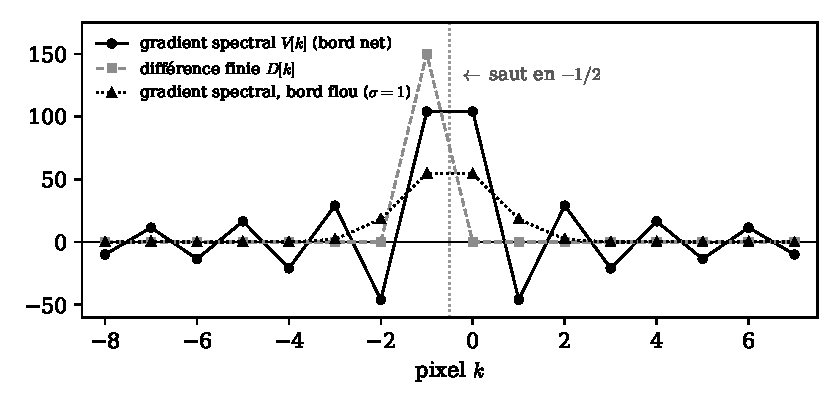
\includegraphics[width=0.78\textwidth]{figures/valeurs.pdf}
\caption{Valeurs aux pixels autour d'un saut de hauteur $H = 150$ situé en $-1/2$. Le gradient spectral oscille en décroissant lentement ; la différence finie vaut $H$ sur un seul pixel et 0 ailleurs ; après un flou ($\sigma = 1$), le gradient spectral devient une bosse sans oscillation.}
\end{figure}
\section*{Pourquoi les ondes ne se compensent pas}
L'intégrale (9) additionne presque toutes les ondes avec le même poids. Sur le pic, elles s'additionnent. Ailleurs, elles se compensent partiellement : l'intégrale s'arrête en $w = \pi$, parce que la grille ne contient pas d'onde plus rapide, et cette coupure brutale laisse un reste $\sin(\pi t) / (\pi t)$. Ce reste s'annule aux distances entières, mais \textbf{les pixels sont à des distances demi-entières du saut} : il ne s'annule jamais.

\section*{Comparaison : la différence finie}
D'après l'outil 1, $\hat{D}(w) = (e^{iw} - 1)\, \hat{f}(w)$. Comme $e^{iw} - 1 = e^{iw}(1 - e^{-iw})$, la formule (7) donne :

\[
\hat{D}(w) = (e^{iw} - 1)\, \frac{H}{1 - e^{-iw}} = H\, e^{iw} .
\]
On revient aux pixels avec l'outil 2, cette fois avec $t = k + 1$ :

\[
D[k] = \frac{H}{2\pi} \int_{-\pi}^{\pi} e^{iw(k+1)}\, dw = H\, \frac{\sin(\pi(k+1))}{\pi(k+1)} .
\]
Ici $k + 1$ est un \textbf{entier} : le sinus s'annule partout, sauf en $k = -1$ où l'expression vaut $H$. Donc $D[-1] = H$ et $D[k] = 0$ pour tous les autres $k$. La différence finie utilise le même ensemble d'ondes, avec des poids constants coupés en $\pi$, mais elle place le pic \textbf{sur le pixel} $-1$, décalé d'un demi-pixel par rapport au vrai saut. Les distances aux autres pixels sont entières, les ondes s'y compensent exactement, et il n'y a aucune oscillation.

\section*{Effet d'un flou}
Un flou gaussien d'écart-type $\sigma$ (en pixels) multiplie chaque coefficient par $e^{-\sigma^2 w^2 / 2}$. Le gradient spectral du saut flouté a donc pour coefficients :

\[
\hat{V}_\sigma(w) = H\, A(w)\, e^{iw/2}\, e^{-\sigma^2 w^2 / 2} .
\]
Pour $\sigma = 1$, le facteur vaut $e^{-\pi^2/2} \approx 0{,}007$ en $w = \pi$ : les poids décroissent jusqu'à presque zéro avant la coupure (figure 1). Il n'y a plus de coupure brutale, la compensation devient presque complète, et le gradient devient une bosse étroite autour du saut, sans oscillation (figure 2). Dans les tests, l'oscillation à 4 pixels du bord passe de 17 à 0,15.

\section*{Ce qu'il faut retenir}
\begin{itemize}
\item La dérivée d'un saut est un pic. Ses coefficients de Fourier sont presque égaux à toutes les fréquences : $\hat{V}(w) = H A(w) e^{iw/2}$, avec $1 \leq A(w) \leq \pi/2$.
\item La grille coupe ces fréquences net en $w = \pi$ : les ondes ne se compensent pas complètement, et il reste $\sin(\pi t)/(\pi t)$ à la distance $t$ du saut.
\item Les pixels sont à une distance demi-entière $t = k + \frac{1}{2}$ du saut, où $\sin(\pi t) = \pm 1$ : $V[k] \approx H (-1)^k / (\pi(k + 1/2))$, des valeurs qui alternent en signe et décroissent en $1/k$.
\item La différence finie échappe aux oscillations en plaçant le pic sur un pixel (distances entières) ; le flou y échappe en adoucissant la coupure en $\pi$.
\item Dans le projet : quand on ne modifie pas le gradient, ces oscillations sont exactement défaites par le solveur (reconstruction à $10^{-13}$). Elles deviennent visibles quand on modifie le gradient dans une zone : en rehaussement de contraste, la moitié du saut ($V[-1]$ ou $V[0]$) est dans la zone sombre et se fait amplifier ; en collage, un masque trop proche d'un contour net coupe ces oscillations, d'où la nécessité d'une marge.
\end{itemize}
\end{document}